\documentclass[french]{article}
\usepackage[utf8]{inputenc}
\usepackage[T1]{fontenc}
\usepackage{babel}
\usepackage{lmodern}
\usepackage{listings}
\usepackage{graphicx}

\title{COMP : Compte rendu TP2}
\author{Aurèle Barrière \& Antonin Garret}
\date{9 décembre 2016}


\begin{document}

\maketitle

\def\refneeded{\texttt{[ref needed]}}
\def\iprint{\textsc{Print}}
\def\iread{\textsc{Read}}
\def\return{\textsc{Return}}

\section{Introduction}
%% une introduction où vous rappeler les objectifs du TP, avec vos propres mots,
Ce projet vise à implémenter la face avant d'un compilateur de VSL \refneeded\ vers du code 3 adresses.
Le but est d'arriver à traiter un langage avec des structures de contrôles, des boucles, des fonctions avec leur prototypes, des appels à des fonctions et des tableaux.

Un parser était déjà fourni et nous a permis de nous concentrer uniquement sur la génération de code 3 adresses depuis un arbre de syntaxe abstrait.


\section{Description de la méthodologie}
%% une description de votre méthodologie de travail (partage des tâches, organisation du code, tests, etc.)
Nous avons implémenté notre compilateur progressivement, de sorte à identifier plus simplement d'éventuelles ereurs. Dans un premier temps, nous ne nous sommes occupés que de la génération de code associé aux expressions arithmétiques. Ensuite, celui du code des expressions et des blocs.

Enfin, il nous a fallu implémenter la génération de code des fonctions et prototypes, puis celle des tableaux.

À chaque étape, nous avons créé des programmes (ou des expressions, ou des instructions) pour tester notre génération. Dans un premier temps, ce code était comparé à celui des exemples dont nous disposions dans le sujet. Ensuite (quand les programmes et les instructions \iprint\ étaient traités), nous avons pu compiler le code 3 adresses en un code exécutable qui permettait de vérifier le comportement.


\section{Bilan du travail réalisé}
%% un bilan de ce qui a été réalisé (complètement/partiellement),
  \subsection{Génération du code d'expressions}
%% une partie existait déjà
  \subsection{Génération du code d'instructions}

  \subsection{Génération du code de programmes}
%% fonctions, prototypes
  \subsection{Vérification de type}
  Enfin, nous avons implémenté un système de vérification de types pour éviter certaines erreurs. En effet, on ne veut pas qu'un programme puisse assigner un tableau à une valeur entière par exemple. Nous avons donc créé une fonction récursive de typage d'expression. Nous avons également dû augmenter le type de la table de symboles, pour qu'un enregistrement retienne aussi son type.

  
\section{Programme d'exemple}
%% un programme VSL de votre cru couvrant toutes les fonctionalités couvertes par votre compilateur,
Nous avons implémenté un programme qui testait la plupart des fonctionnalités de notre compilateur, et tel qu'on puisse vérifier facilement la correction. Nous avons donc choisi un programme qui décrit la fractale du \textit{tapis de Sierpinski} \refneeded. Comme nous n'avions pas accès à des primitives de dessin, le programme se contente d'afficher dans la sortie standard (avec des \iprint) les coordonnées de chaque carré à colorier (un angle du carré et une longueur). Un programme écrit en \textsc{Python} se charge ensuite de dessiner ces carrés.

Le programme utilise des prototypes de fonctions, des fonctions avec arguments, des appels récursifs, des conditions \texttt{IF} sans \texttt{ELSE}, des expressions arithmétiques passées en paramètres de fonctions, des divisions et un retour dans une fonction de type \textsc{Void}.

Le programme \textsc{VSL} :
\lstinputlisting{../tests/sierpinski.vsl}


Le programme \textsc{Python} chargé d'afficher le résultat :
\lstinputlisting[language=Python]{../plot.py}

Et le résultat :

\begin{center}
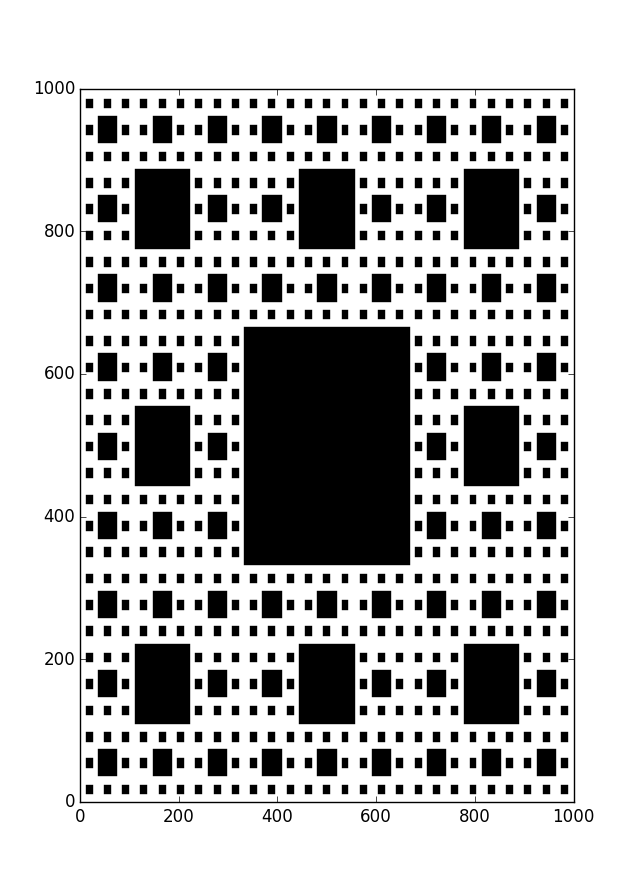
\includegraphics[width=10cm, height=10cm]{../sierpinski.png}
\end{center}

Nous avons également écrit un script qui compile notre programme, l'exécute en écrivant sa sortie dans un fichier, puis appelle le programme \textsc{Python} pour créer l'image. Pour simplifier le programme, les valeurs de rang maximal et de longueur du carré initial sont écrite directement dans le code. Si des petites irrégularités se distinguent dans la figure, elles s'expliquent par le fait que nos programmes n'utilisent que des variables entières et il y a donc quelques problèmes d'arrondi.

\section{Tests effectués}
%% un rapport des tests que vous avez effectués (voir fichiers VSL de test sur le share),
Nous avons commencé par créer un script en \textsc{Bash} qui affichait les programmes de tests puis les compilait, puis les exécutait pour automatiser le lancement des tests.

Une fois que notre compilateur générait du code pour les programmes, nous avons pu lancer les tests fournis avec le sujet. Ceux-ci nous ont permis de vérifier que notre gestion des blocs, fonctions, prototypes, tableaux... était correcte.

Ils nous ont également permis de soulever un problème de notre implémentation : les instructions \return\ dans les fonctions de type \textsc{Void}. Dans une première version, nous avions décidé que les programmes qui essayaient de retourner une valeur dans un programme de type \textsc{Void} n'étaient pas corrects et ne devaient pas être compilés. Cependant, de nombreux programmes de tests le faisaient, puisqu'il n'y pas d'instruction \return\ sans argument en VSL. Nous avons donc modifié notre compilateur pour qu'un tel appel crée une intruction \texttt{ret void} dans le code 3 adresses généré.

\section{Conclusion}
%% une conclusion où vous discuterez des difficultés rencontrées, de ce  que vous avez appris, etc.
Dans ce projet, nous avons appris à implémenter un générateur de code 3 adresses.

Notre implémentation progressive et l'utilisation de nombreux programmes de tests nous ont permis de détecter le plus tôt possible nos erreurs.

La possibilité de compiler nos programmes nous a donné une moyen efficace de vérifier chaque fonctionnalité de notre compilateur.

Quelques problèmes se sont posés pendant notre implémentation : blocs vides en cas de \texttt{IF} sans \texttt{ELSE}, retour dans les fonctions de type \textsc{Void}, blocs vides en fin de fonction, mauvaise gestion des paramètres des fonctions (pour résoudre ce problème, nous avons créé pour chaque paramètre une variable locale dans laquelle on copiait sa valeur).

Cependant, tous ces problèmes ayant étés corrigés, nous avons un compilateur qui produit du code se comportant comme attendu pour chaque problème de test correct, et qui ne compile pas pour chaque problème de test d'erreur.
\end{document}
